\subsection{Module Implementation}

The code can be found in the attachments.

\textbf{Entity}

The ports of the modules are taken from the block diagram in figure \ref{fig:delay}. The in- and output can be determined from the arrow directions.

\textbf{Architectures}

\textit{Counter-Architecture:}

\begin{quote}
    The counter architecture consists of a signal, which is used to increment the actual counter output. A register process handles the reset and clock behaviour: On reset, the counter output is set to $0$. On each rising edge of the clock signal, the sychronous counter reset strobe is checked. If the strobe is set, the counter is set to $0$, else the counter is incremented by one.
\end{quote}

\textit{Statemachine-Architecture}

\begin{quote}
    The functionality of the statemachine is described by two processes: One register process describes the clock and reset behaviour. Here, the state variable is updated every clock cycle. Another combinatorial process determines the next state. Here the counter period can be set by editing the \lstinline{MAX_COUNT} constant.
\end{quote}

\textbf{Test-Bench}

Before the stimulus process a clock oscillation is emulated and a reset is performed. To test the module implementations, two scenarios are tested:

\begin{itemize}
    \item Pressing the start button at different timestamps
    \item Performing a synchronous reset
\end{itemize}

\newpage

\subsection{Simulation}

\textbf{Start Button Stimulus}

A single start pulse triggers the statemachine:
\begin{center}
    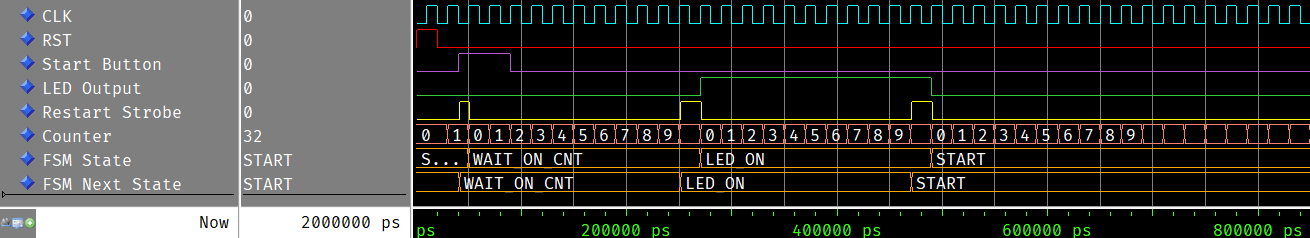
\includegraphics[width=\textwidth]{images/SimP2_1.png}
\end{center}

Any further start button press have no effect during the \lstinline{WAIT} and the \lstinline{LED_ON} state.
\begin{center}
    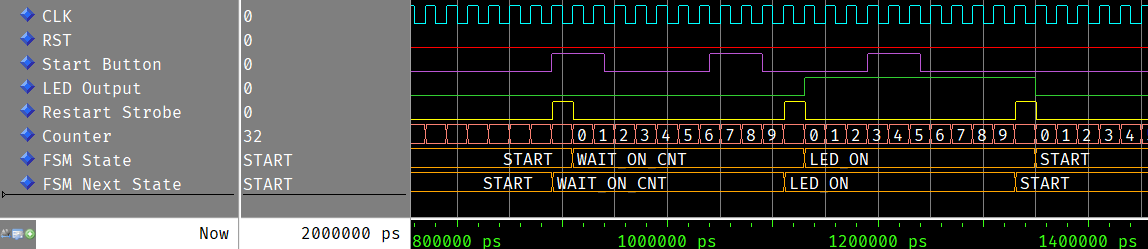
\includegraphics[width=\textwidth]{images/SimP2_2.png}
\end{center}

\textbf{Reset Stimulus}

The waveform shows, that a synchronous reset during the \lstinline{WAIT} and \lstinline{LED_ON} cancels the blinking process of the led.

\begin{center}
    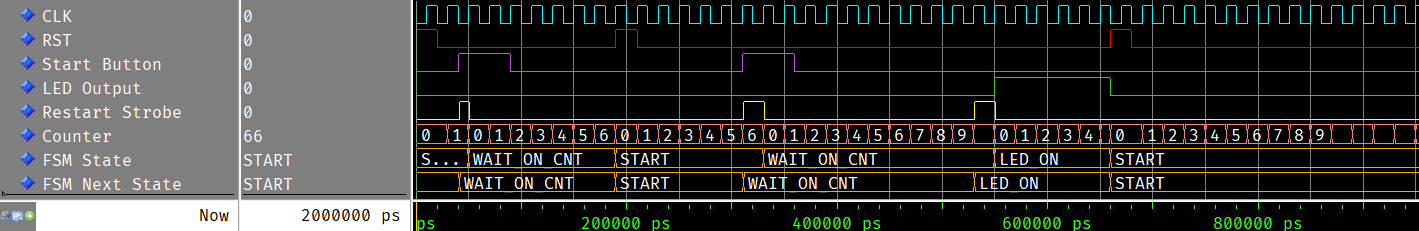
\includegraphics[width=\textwidth]{images/SimP2_3_Reset.png}
\end{center}

\textbf{Results} 

Because the outputs are purely dependent on the states themselves and not on any other inputs, the fsm is per definition a mealy machine.
